\documentclass[]{article}
\usepackage{lmodern}
\usepackage{amssymb,amsmath}
\usepackage{ifxetex,ifluatex}
\usepackage{fixltx2e} % provides \textsubscript
\ifnum 0\ifxetex 1\fi\ifluatex 1\fi=0 % if pdftex
  \usepackage[T1]{fontenc}
  \usepackage[utf8]{inputenc}
\else % if luatex or xelatex
  \ifxetex
    \usepackage{mathspec}
  \else
    \usepackage{fontspec}
  \fi
  \defaultfontfeatures{Ligatures=TeX,Scale=MatchLowercase}
\fi
% use upquote if available, for straight quotes in verbatim environments
\IfFileExists{upquote.sty}{\usepackage{upquote}}{}
% use microtype if available
\IfFileExists{microtype.sty}{%
\usepackage{microtype}
\UseMicrotypeSet[protrusion]{basicmath} % disable protrusion for tt fonts
}{}
\usepackage[margin=1in]{geometry}
\usepackage{hyperref}
\hypersetup{unicode=true,
            pdftitle={Increased Levels of Microplastics Found in Urban Freshwater Lake},
            pdfauthor={Christian Clark and Claire Generous, EA030- Environmental Science, Pomona College Environmental Analysis Department},
            pdfborder={0 0 0},
            breaklinks=true}
\urlstyle{same}  % don't use monospace font for urls
\usepackage{color}
\usepackage{fancyvrb}
\newcommand{\VerbBar}{|}
\newcommand{\VERB}{\Verb[commandchars=\\\{\}]}
\DefineVerbatimEnvironment{Highlighting}{Verbatim}{commandchars=\\\{\}}
% Add ',fontsize=\small' for more characters per line
\usepackage{framed}
\definecolor{shadecolor}{RGB}{248,248,248}
\newenvironment{Shaded}{\begin{snugshade}}{\end{snugshade}}
\newcommand{\AlertTok}[1]{\textcolor[rgb]{0.94,0.16,0.16}{#1}}
\newcommand{\AnnotationTok}[1]{\textcolor[rgb]{0.56,0.35,0.01}{\textbf{\textit{#1}}}}
\newcommand{\AttributeTok}[1]{\textcolor[rgb]{0.77,0.63,0.00}{#1}}
\newcommand{\BaseNTok}[1]{\textcolor[rgb]{0.00,0.00,0.81}{#1}}
\newcommand{\BuiltInTok}[1]{#1}
\newcommand{\CharTok}[1]{\textcolor[rgb]{0.31,0.60,0.02}{#1}}
\newcommand{\CommentTok}[1]{\textcolor[rgb]{0.56,0.35,0.01}{\textit{#1}}}
\newcommand{\CommentVarTok}[1]{\textcolor[rgb]{0.56,0.35,0.01}{\textbf{\textit{#1}}}}
\newcommand{\ConstantTok}[1]{\textcolor[rgb]{0.00,0.00,0.00}{#1}}
\newcommand{\ControlFlowTok}[1]{\textcolor[rgb]{0.13,0.29,0.53}{\textbf{#1}}}
\newcommand{\DataTypeTok}[1]{\textcolor[rgb]{0.13,0.29,0.53}{#1}}
\newcommand{\DecValTok}[1]{\textcolor[rgb]{0.00,0.00,0.81}{#1}}
\newcommand{\DocumentationTok}[1]{\textcolor[rgb]{0.56,0.35,0.01}{\textbf{\textit{#1}}}}
\newcommand{\ErrorTok}[1]{\textcolor[rgb]{0.64,0.00,0.00}{\textbf{#1}}}
\newcommand{\ExtensionTok}[1]{#1}
\newcommand{\FloatTok}[1]{\textcolor[rgb]{0.00,0.00,0.81}{#1}}
\newcommand{\FunctionTok}[1]{\textcolor[rgb]{0.00,0.00,0.00}{#1}}
\newcommand{\ImportTok}[1]{#1}
\newcommand{\InformationTok}[1]{\textcolor[rgb]{0.56,0.35,0.01}{\textbf{\textit{#1}}}}
\newcommand{\KeywordTok}[1]{\textcolor[rgb]{0.13,0.29,0.53}{\textbf{#1}}}
\newcommand{\NormalTok}[1]{#1}
\newcommand{\OperatorTok}[1]{\textcolor[rgb]{0.81,0.36,0.00}{\textbf{#1}}}
\newcommand{\OtherTok}[1]{\textcolor[rgb]{0.56,0.35,0.01}{#1}}
\newcommand{\PreprocessorTok}[1]{\textcolor[rgb]{0.56,0.35,0.01}{\textit{#1}}}
\newcommand{\RegionMarkerTok}[1]{#1}
\newcommand{\SpecialCharTok}[1]{\textcolor[rgb]{0.00,0.00,0.00}{#1}}
\newcommand{\SpecialStringTok}[1]{\textcolor[rgb]{0.31,0.60,0.02}{#1}}
\newcommand{\StringTok}[1]{\textcolor[rgb]{0.31,0.60,0.02}{#1}}
\newcommand{\VariableTok}[1]{\textcolor[rgb]{0.00,0.00,0.00}{#1}}
\newcommand{\VerbatimStringTok}[1]{\textcolor[rgb]{0.31,0.60,0.02}{#1}}
\newcommand{\WarningTok}[1]{\textcolor[rgb]{0.56,0.35,0.01}{\textbf{\textit{#1}}}}
\usepackage{graphicx,grffile}
\makeatletter
\def\maxwidth{\ifdim\Gin@nat@width>\linewidth\linewidth\else\Gin@nat@width\fi}
\def\maxheight{\ifdim\Gin@nat@height>\textheight\textheight\else\Gin@nat@height\fi}
\makeatother
% Scale images if necessary, so that they will not overflow the page
% margins by default, and it is still possible to overwrite the defaults
% using explicit options in \includegraphics[width, height, ...]{}
\setkeys{Gin}{width=\maxwidth,height=\maxheight,keepaspectratio}
\IfFileExists{parskip.sty}{%
\usepackage{parskip}
}{% else
\setlength{\parindent}{0pt}
\setlength{\parskip}{6pt plus 2pt minus 1pt}
}
\setlength{\emergencystretch}{3em}  % prevent overfull lines
\providecommand{\tightlist}{%
  \setlength{\itemsep}{0pt}\setlength{\parskip}{0pt}}
\setcounter{secnumdepth}{0}
% Redefines (sub)paragraphs to behave more like sections
\ifx\paragraph\undefined\else
\let\oldparagraph\paragraph
\renewcommand{\paragraph}[1]{\oldparagraph{#1}\mbox{}}
\fi
\ifx\subparagraph\undefined\else
\let\oldsubparagraph\subparagraph
\renewcommand{\subparagraph}[1]{\oldsubparagraph{#1}\mbox{}}
\fi

%%% Use protect on footnotes to avoid problems with footnotes in titles
\let\rmarkdownfootnote\footnote%
\def\footnote{\protect\rmarkdownfootnote}

%%% Change title format to be more compact
\usepackage{titling}

% Create subtitle command for use in maketitle
\providecommand{\subtitle}[1]{
  \posttitle{
    \begin{center}\large#1\end{center}
    }
}

\setlength{\droptitle}{-2em}

  \title{Increased Levels of Microplastics Found in Urban Freshwater Lake}
    \pretitle{\vspace{\droptitle}\centering\huge}
  \posttitle{\par}
    \author{Christian Clark and Claire Generous, EA030- Environmental Science,
Pomona College Environmental Analysis Department}
    \preauthor{\centering\large\emph}
  \postauthor{\par}
      \predate{\centering\large\emph}
  \postdate{\par}
    \date{5/12/2019}


\begin{document}
\maketitle

\hypertarget{abstract}{%
\subsection{Abstract}\label{abstract}}

Increased use of single use plastics and other plastic products has led
to the emergence of plastics in the environment as a dangerous new type
of pollution. Plastics in ecosystems can have negative impacts on human
health, ecosystem health, and biodiversity. Little is currently known
about the concentrations of microplastics (plastics \textless{} 5mm) in
freshwater systems, but there are already concerns about the effects
they may have on the health of marine and aquatic ecosystems. We sought
to fill in knowledge gaps about microplastics in freshwater systems. We
found that a fresh water lake in an urban environment had significantly
higher concentrations of microplastics than tap water. This has
implications for other urban freshwater reservoirs- such as polluted
drinking water and food- used by humans as well as other freshwater
systems important for biodiversity and ecosystem function across the
world.

\hypertarget{introduction}{%
\subsection{Introduction}\label{introduction}}

Significance

Microplastics come from almost all plastic products used by humans and
can be found in water, soil, and even in the air. They can also have
impacts on human health, as well as on numerous ecosystems, even being
as poisoning and killing marine life (Karbalaei et al.~2018). When not
properly disposed of, plastics can break down into toxic chemicals that
bioaccumulate and enter the food chain, poisoning and possibly killing
many organisms ranging from plants all the way up to humans (Huerta et
al.~2017). In urban areas, the contamination can be high, with levels of
microplastics in waste water being seen at 260-320 x 103 particle m-3 in
cities such as Paris (Dris et al.~2015). As utilization of single-use
plastics increase, concern about microplastics in food and water sources
is rising (Koelmans et al.~2019). This added to the significance of the
study of microplastics in urban environments. In order to improve
mitigation strategies for microplastics in human-consumed products,
research must be done to determine concentrations in treated tap water
and untreated fresh water. While seeking to fill in knowledge gaps about
microplastics in freshwater systems, we hypothesized that microplastic
levels would be higher in the local body of fresh water than in tap
water, which may in turn lead to bioaccumulation of microplastics
throughout the surrounding habitat and region.

\begin{Shaded}
\begin{Highlighting}[]
\KeywordTok{summary}\NormalTok{(cars)}
\end{Highlighting}
\end{Shaded}

\begin{verbatim}
##      speed           dist       
##  Min.   : 4.0   Min.   :  2.00  
##  1st Qu.:12.0   1st Qu.: 26.00  
##  Median :15.0   Median : 36.00  
##  Mean   :15.4   Mean   : 42.98  
##  3rd Qu.:19.0   3rd Qu.: 56.00  
##  Max.   :25.0   Max.   :120.00
\end{verbatim}

Current Literature and Known Techniques

The analysis of microplastics in water is a process that can be complex
due to their ubiquitous presence (Liu et al.~2019). As such, techniques
are different depending on the sizes of the microplastics that
researchers seek to identify, however there were a few main techniques
that are more widely used by researchers. To preliminarily obtain the
plastics there were three main methods, selective, bulk, and volume
reducing sampling (Wang and Wang 2018). For the purposes of our project
we will use bulk sampling of water as it is the most appropriate method
for comparing plastics in these water sources (Wang and Wang 2018).
There were also many ways to analyze and identify plastics after
obtaining them. For example, larger microplastics can be visually
identified with a microscope or other visual aid, though only after
going through a wet sieve process to separate the water from the solid
matter (Masura et al.~2015). For many studies, visual identification is
not enough because plastics may not be visible to the naked eye, so
additional measures are taken. The main method found in much of the
literature today is outlined in Masura's guide for analysis of
microplastics in water. This involves a wet sieve, followed by
determining the mass of total solids, wet peroxide oxidation (WPO), with
subsequent density separation and microscope identification (Masura et
al 2015). This method was used in a study that found microplastic
concentrations in Canada's Lake Winnipeg to be equal to or greater than
those in the Great Lakes basin (Anderson et al.~2017). Another technique
widely used is infrared spectroscopy. This technique entails filtering a
water sample using a vacuum set up through a filter paper and
subsequently staining and drying the paper. After this, the paper is put
under an infrared microscope and particles are identified. The
limitation with this technique is its inability to identify particles
less than 20 µm, for which a different type of spectroscopy is needed
(Schymanski et al.~2018). If these technologies are not available,
optical techniques using microscopes and dyes are common for
identification (Wang and Wang 2018). For this project, we decided to use
this optical technique using red dye, and infrared light, and a
microscope. This method was the most plausible given the resources
available to us, as well as the budgetary and time constraints placed
upon this project. Additionally, we have experience with this technique
already, allowing us to possibly reduce human error in data collection
and analysis.

Knowledge Gaps

Though microplastics have been studied in aquatic environments, most of
the current literature is focused on marine environments, with much less
being known about freshwater biomes (Su et al.~2016). Additionally, not
much is known about the mechanisms by which microplastics bioaccumulate
and the extent of their impact aquatic life in freshwater systems, their
greater ecosystems, and human health (Eerkes-Medrano et al.~2015)
(Koelmans et al.~2019). By researching a freshwater lake, we hope to
contribute more knowledge to these areas. Since there is not a lot of
research on urban freshwater lakes and microplastics, there is a lack of
literature about microplastics in freshwater in areas surrounded by
urbanization. Even more comprehensive reviews of lakes and their water
quality (which would include microplastics) do not really talk about
manmade lakes and how they compare to the surrounding ecosystem
(Bhateria and Jain 2016). This knowledge gap surrounding man-made lakes
is something we aimed to address, as artificial lakes do impact the
local ecosystem, and perhaps human life in the area. By looking at
artificial lakes, we can see how human development is contributing to
plastic pollution and possibly to endangered native ecosystems and the
organisms that inhabit them. This research is important to contribute to
our understanding of how urbanization can have impacts on plastic
prevalence in both native ecosystems and human society.

Research Question and Hypothesis

The question we aimed to answer in this study was whether there are
differences in treated vs untreated freshwater microplastic
concentrations. Based on studies in the existing literature, we
hypothesized that the untreated freshwater from pHake lake (located in
the Bernard Field Station in Claremont, CA) would have a higher number
of microplastics than the treated water from the Claremont Colleges
(Dris et al.~2015, Anderson et al.~2017).

Research Approach

There are multiple steps needed in order to ensure an accurate
representation of plastic contents in both pHake lake and the water
system in Claremont. We employed a bulk sampling method, taking one
sample from pHake Lake and one from an on-campus water fountain, with
each location having 10 replicate samples.(Wang and Wang 2018). Samples
from the lake were taken in approximately the middle of pHake lake at a
depth of 2 meters below surface using a depth sampler. Two meters
represents the relative middle in terms of depth in pHake Lake. Samples
were collected in 1L glass vials to avoid any cross-plastic
contamination. The water was then mixed with 1 mg/mL Nile Red dye and
incubated for 30 minutes. Water was filtered using a vacuum filter and
filter paper. Blanks were made for quality control purposes. After
filtration, samples were analyzed using an Echo Revolve RVL-100-B
microscope and red LED infrared light.

Plastic Quantification

To quantify the plastics, we will use the microscope and infrared light
to enumerate microplastics on random sections of the filter paper. To
avoid biases, the filter paper will be split into sections and numbered
before identification. The section to be observed will be determined by
using the random number generator on the open source statistical
analysis program R. This will be repeated three times per sample. We
will then record and then average the number of microplastics seen in
samples from pHake Lake, treated water from campus, and our blanks.
Because of differences in weather patterns on sample collection days, as
well as daily fluctuations in foot and motor traffic along the borders
of the sites, we expect our data to have some variation. Current
literature, unfortunately, is not comprehensive enough to give any
indication of a range of values to expect, but we do expect more
plastics to be in the lake water than tap water.

Statistical Analysis

As the data collected was discrete, we used a one-tailed t-test to
examine any difference between the means of the treatments. The t-tests
were carried out between the pHake Lake samples and treated water
samples. Results have been compiled and presented in tables and figures
below so that they may be easily understood by all, regardless of
scientific background.

Results To quantify the microplastics in each of our samples, we divided
each filter paper in 8 sections and chose three at random to count the
number of plastics. All objects larger than 400 micrometers were
disregarded during observation. The water from pHake Lake, had a higher
average microplastic concentration per sector than both the campus water
and the blank (Table 1). Each Sector is about 1/8 of the filter paper.
This means that sector averages need to be multiplied by 8 to get the
average number of micro plastics per 500mL of water. For Lake water,
this number is 114.9 microplastics and for campus water this number is
30.91 microplastics per 500mL water with 2.64 microplastics for the
blank. A t-test was used to determine if there was any significance
between our two treatment groups. This test showed our results to be
highly significant (p \textless{}.01), meaning that there is almost no
way the difference in microplastic concentrations between our two sites
is random or natural. Figure 1 shows a boxplot of average number of
microplastics per sector of filter paper for both treatment groups. As
such, we can conclude that there are factors (most likely anthropogenic)
that are leading to increased levels of microplastics in pHake Lake and
possibly the Bernard Field Station as a whole.

Table 1: Average Number of Microplastics Per Sector

Lake Water Campus Water Blank 14.36 3.864 0.333

\includegraphics{fullsizeoutput_ale.jpeg} {[}\emph{\textbf{Figure 1.}
Average Microplastic Concentration by Site}{]}

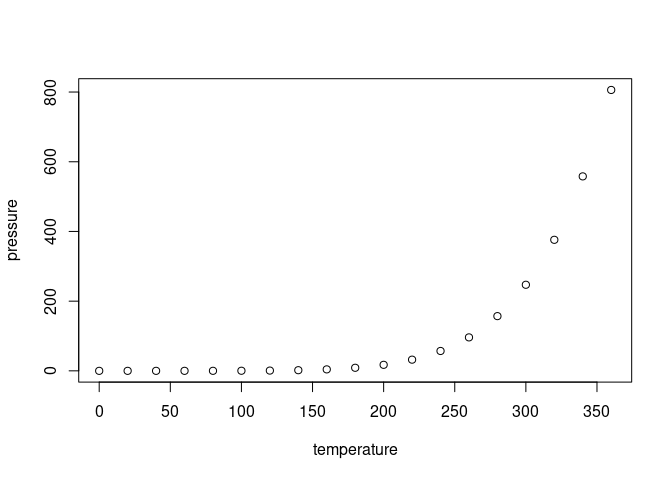
\includegraphics{Plastics_Report_files/figure-latex/pressure-1.pdf}

Note that the \texttt{echo\ =\ FALSE} parameter was added to the code
chunk to prevent printing of the R code that generated the plot.


\end{document}
